\section{Introduction}
I have spent the majority of my time this week improving my Long - Short Term Memory network (PyTorch version), trying to extract videos' features by using TensorHub Module\cite{tensorhub} and TensorFlow for Poets\cite{tf4poets}. As mentioned before, till this week I would only work with the Short-term subtask so all my experiments from this moment were performed on the Short-term memorability scores.

\section{Feature Extracting}
\subsection{Using TensorHub}
In week 9, I had already try to extract images' features but at that moment I misunderstood the concept of how TensorFlow actually worked. After learning more about how to use TensorFlow this week I finally figured out how to use TensorHub to extract features correctly.

I used TensorHub to extract images' features with pretrained Inception V3 network. As mentioned by TensorHub, the checkpoint exported into the module was inception-v3-2016-08-28/inception-v3.ckpt downloaded from \href{https://github.com/tensorflow/models/blob/master/research/slim/README.md#pre-trained-models}{TensorFlow-Slim's pre-trained models}. Its weights were originally obtained by training on the ILSVRC-2012-CLS dataset for image classification (Imagenet).

All my code could be found on my \href{https://colab.research.google.com/drive/1mL2fH6zuTS-8o1Z6oKtmF1Mt-6f32LsX}{Colab notebook}. I also normalized the input image by subtracting it by \textbf{\emph{128}} then dividing it by \textbf{\emph{128}} (IMPORTANT step). This module took me more than one hour to extract 8000 videos (8 frames for each video), which were around 64000 frames total.

\subsection{Using TensorFlow for Poets}
TensorFlow provided a tutorial called TensorFlow for Poets teaching how use transfer learning, which meant starting with a model that had been already trained on another problem, then retrain it on a similar problem.

At the 4th step Retraining the network, they described correctly how their retrain script worked. I changed the architecture argument to Inception V3 to use it as pretrained model to extract bottleneck values. 

One of the very first phase of their retrain script  was to analyzed all the images and calculated the bottleneck values for each of them. The term bottlen-eck here was actually indicated the term feature. After this phase I got a folder containing all images' bottleneck values, the next job I had to do was concatenating them all to work later.

\section{PyTorch LSTM Classification Network}
\subsection{Architecture}
Beside using the same architecture as I had used in week 9, I added 2 Fully-Connected Layers separately to initialize the hidden state \textbf{\emph{h0}} and cell state \textbf{\emph{c0}} of the LSTM cells based on the input. The motivation behind this change was when I thought using a randomly initialized hidden state and cell state was nothing but a terrible idea because it made no sense at all.

These 2 Fully-Connected Layers I mentioned above turned the input size of [batch-size, sequence-length, input-size] (e.g. [1000, 8, 2048]) to hidden state and cell state sizes of [num-layers, batch-size, hidden-size] (e.g. [3, 1000, 1024]).

\subsection{Training on Dev-Set (extracted by Inception V3 with TensorFlow for Poets)}
\subsubsection{Strategy}
Till this moment I would use this strategy for every new networks. I splitted the provided Dev-Set for this challenge into three parts, since the Dev-Set had 8000 videos, I picked \textbf{\emph{6000}} videos for training, \textbf{\emph{1000}} videos for validating and the last \textbf{\emph{1000}} videos for testing.

\subsubsection{Version 2.1}
As described above in the architecture section, I used my version 2 architecture powered by some Fully-Connected Layers so I called this 2.1. I trained this architecture with only \textbf{\emph{100}} epochs and at the learning rate of \textbf{\emph{1e-4}}. My network converged with only around 50 epochs and the loss value seemed to decreasing stably.

The best correlation value on Validate set was \textbf{\emph{0.4757}} and the minimum loss value was \textbf{\emph{0.011}}. As the loss would continue decreasing, the correlation value also decreased, so I thought it was over-fitting.

\begin{figure}[!ht]
\centering
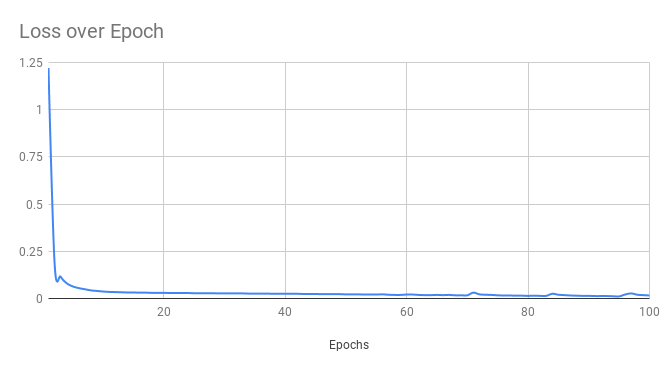
\includegraphics[width=\textwidth]{week14-devset-tf-v2-1-loss.png}
\caption{Loss over Epoch (on Train set).}
\end{figure}

\newpage
\begin{figure}[!ht]
\centering
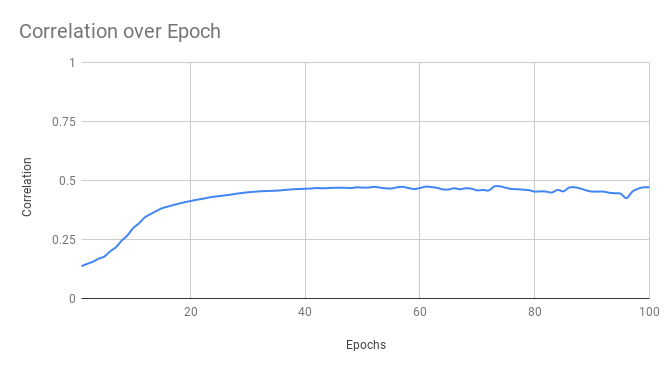
\includegraphics[width=\textwidth]{week14-devset-tf-v2-1-correl.png}
\caption{Correlation over Epoch (on Validate set).}
\end{figure}

Lately, I used this pre-trained model to calculate the correlation value on the test, the correlation was a little bit lower but acceptable, which was \textbf{\emph{0.4591}}.

\subsection{Training on Dev-Set (extracted by Inception V3 with TensorHub)}
\subsubsection{Version 2.1}
I trained this architecture with only \textbf{\emph{100}} epochs and at the learning rate of \textbf{\emph{1e-4}}.

\begin{figure}[!ht]
\centering
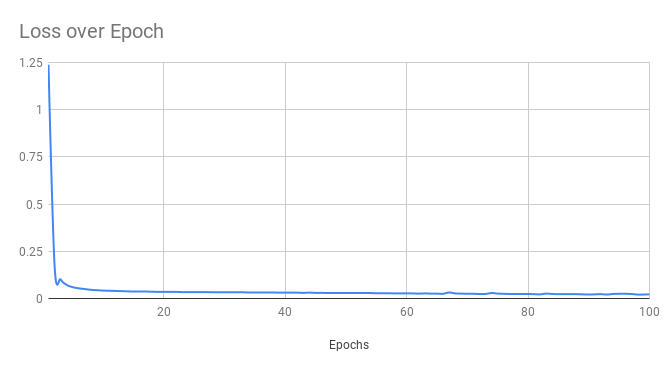
\includegraphics[width=\textwidth]{week14-devset-th-v2-1-loss.png}
\caption{Loss over Epoch (on Train set).}
\end{figure}

The best correlation value on Validate set was \textbf{\emph{0.3585}} and the minimum loss value was \textbf{\emph{0.021}}. As the loss would continue decreasing, the correlation value also decreased, so I thought it was over-fitting.

\begin{figure}[!ht]
\centering
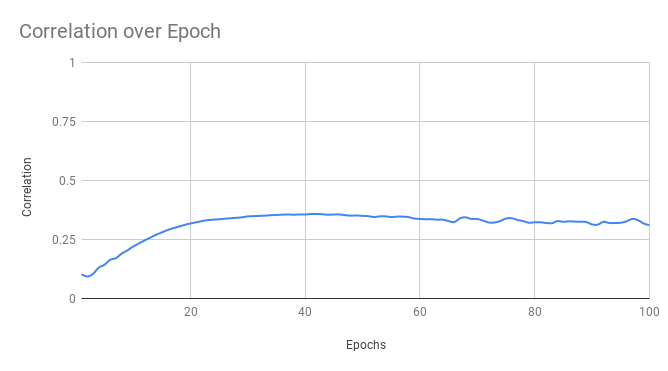
\includegraphics[width=\textwidth]{week14-devset-th-v2-1-correl.png}
\caption{Correlation over Epoch (on Validate set).}
\end{figure}

Then I used this pre-trained model to calculate the correlation value on the test, the correlation was a little bit lower but acceptable, which was \textbf{\emph{0.2989}}.

\subsubsection{Comment}
I did not normalized the images before extracting their feautures in the previous week, and the value of correlation on Validate set was only 0.2x; the value of correlation on Test set was even worse (0.01x).

In this week I tried normalizing the images and my features performed much more better. The results was described above in the sub section above.